\textbf{VII -- GLI ALFIERI}

Un ruolo particolare ricoprono gli Alfieri. Siccome un Alfiere gioca
solo su metà scacchiera il cambio di uno di essi significa un controllo
minore sulle case del colore che l'Alfiere occupa. Da qui la necessità
di valutare correttamente un eventuale cambio.

\textbf{a) La coppia degli Alfieri}

Possedere entrambi gli Alfieri mentre l'avversario ne ha uno solo o
nessuno (cambiati con i Cavalli) può costituire un vantaggio. Dico
\emph{può} perché abbiamo imparato quanto il valore del materiale sia
relativo alla sua disposizione sulla scacchiera e dipenda molto da
fattori quali la coordinazione dei pezzi, la struttura dei pedoni,
l'occupazione di case o colonne, ecc. La coppia degli Alfieri si
valorizza nelle posizione aperte, posizioni in cui i pedoni non siano di
intralcio alla loro azione. Ne consegue che chi si trova ad avere il
vantaggio della coppia degli Alfieri deve aprire il gioco cambiando i
pedoni, specie quelli centrali. In caso di lunghe catene di pedoni non
mobili, invece, i Cavalli in genere valgono più dei due Alfieri.

Furman--Lipnizky, Kiev 1951 \textbf{(Difesa Nimzo Indiana)}

\textbf{1.d4 ¤f6 2.c4 e6 3.¤c3 ¥b4 4.e3} molto giocata è anche la
variante Capablanca (4.£c2) con cui il Bianco evita la formazione di un
pedone doppiato dopo il cambio in c3.

\textbf{4... 0-0 5.¥d3 d5 6.¤f3 £xc4 7.¥xc4 ¤c6 8.0-0 ¥d6} le ultime due
mosse manifestano la volontà del Nero di eseguire la spinta in e5, utile
a dare spazio all'¥c8.

\textbf{9.¥b5} giocata per impedire tale spina che ora costerebbe un
pedone.

\textbf{9... e5!} Lipnizky non si tira indietro in considerazione che
l'apertura delle linee, in presenza della coppia degli Alfieri, è un
compenso sufficiente.

\textbf{10.¥xc6 exd4 11.¥xb7 ¥xb7 12.¤xd4 £d7 13.¤db5 £c6 14.f3}

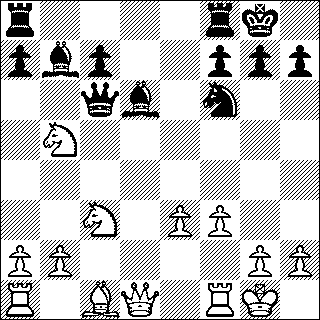
\includegraphics[width=1.5in,height=1.5in]{assets/diagrams/image94.png}

\emph{diagramma 94}

È sempre interessante vedere come hanno ragionato i giocatori nei
momenti critici della partita. Ecco il pensiero di Lipnizky su questa
posizione:

``Furman si sentiva a suo agio. Cerchiamo di capire cosa può aver
pensato. Le conseguenze più immediate del suo guadagno di pedone sono
state:

\emph{1) Nel territorio del Bianco sono comparse molte case deboli;}

\emph{2) I pezzi bianchi dell'ala di Donna non sono sviluppati.}

Valutando la situazione da questo punto di vista, 14.f3 assume un
significato specifico: infatti, non solo provvede ad eliminare l'attacco
in g2 da parte della batteria \textbf{£}+\textbf{¥} del Nero,
limitandone l'azione sulla diagonale a8 hl, ma prepara anche la spinta
in e4 per cercare di ultimare lo sviluppo ad ovest. Inoltre, ponendo i
propri pedoni su case bianche, si cerca di ovviare alla mancanza
dell'Alfiere campochiaro. D'altro canto, il Nero ha già completato la
collocazione ottimale dei suoi pezzi, ed ha l'iniziativa. Se il Bianco
riuscisse però a portare a compimento il suo piano, è indubbio che ci
sarebbe un ben scarso compenso per il pedone.

\emph{Qual è allora il modo migliore di aumentare e consolidare il
vantaggio, partendo dal presupposto che non dispongo di un attacco
contro il Re? La risposta a questo quesito chiama in causa il concetto
secondo il quale bisogna, in primo luogo, impedire che il piano nemico
si realizzi. Ecco lo scopo delle mie prossime mosse''.}

\textbf{14... ¥e5 15.£c2 ¦fd8 16.a4} il Bianco poteva restituire il
pedone e rimettere in gioco i pezzi con 16..¤d4 ¤xd4 17.exd4 ¦xd4
18.¥e3.

\textbf{16... £c4} minaccia £h4.

\textbf{17.£f2 ¦d3 18.¢h1 ¦ad8 19.e4 a6 20.¤a3 £d3 21.} ¤\textbf{ab1}
merita considerazione 21.¥e3 per recuperare lo svantaggio di sviluppo se
il Nero si riprende il pedone dopo 21... ¥xc3.

\textbf{21... ¥d4} il trasferimento di questo Alfiere sulla diagonale
a7-g1 si rivelerà decisivo.

\textbf{22.£e2 ¥c5} impedisce ¦a3.

\textbf{23.¦e1 a5 24.¤d2 £c2! 25.¤f1 £xe2 26.¦xe2 ¦d1} Lipnizki
commenta: \emph{``Lo sfondamento decisivo avviene sulle case bianche in
precedenza indebolite dalle manovre £d7-c6-c4-b3-c2, e ¦d8-d3-d1. Si
guadagneranno ora due pezzi per la Torre''.}

\textbf{27.¤xd1 ¦xd1 28.h3 ¦xf1+ 29.¢h2 ¥g1+ 30.¢g3 ch5+ 31.¢g4 g6 32.b4
¥d4 33.¥b2 ¥xb2 34.¦xf1 ¥c8+} e il Re non sfugge alla rete di matto.

\textbf{35.¢g5 ¥f6 36.¢h6 ¤f4} con l'idea ¤e6 e matto d'Alfiere in g7 o
g5.

\textbf{36.} il Bianco abbandona.

\emph{diagramma 95}

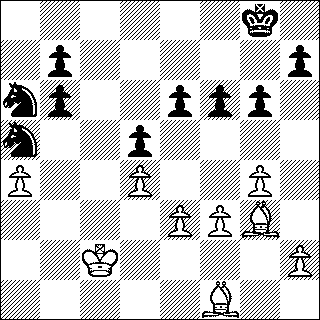
\includegraphics[width=1.5in,height=1.5in]{assets/diagrams/image95.png}

Il vantaggio della coppia degli Alfieri non si limita al centro partita
ma è valido anche in finale. Nella decima partita del campionato del
mondo del 1955 tra Botvinnik e Bronstein, dopo la 37\textsuperscript{a}
mossa si raggiunse la posizione del diagramma.

Il pedone in più del Nero non è significativo a causa della doppiatura.
Potrebbe essere valorizzato in un finale di Cavallo contro Alfiere ma il
Bianco si guarda bene da cambiare uno dei suoi gioielli; anche con un
pedone in meno il Bianco gioca per vincere.

\textbf{38.¢c3 ¢f7 39.e4 f5} un errore. Aprire le linee favorisce chi
possiede i due Alfieri.

\textbf{40.gxf5 gxf5 41.¥d3 ¢g6} la doppia presa in e4 costa la partita
a causa di un bel sacrificio d'Alfiere che permette la penetrazione del
Re sul lato di Donna. 41... £xe4 42.fxe4 fxe4 43.¥xe4 ¢g7 44.¥xb7!! ¤xb7
45.¢c4 e il ¤a6 non ha case di fuga.

\textbf{42.¥d6} Botvinnik perde l'occasione di assestare il colpo di
grazia con 42.¥b1. Dopo tale mossa con 42... fxe4 si rientra nella
variante esaminata nella nota precedente mentre dopo 42... ¤c4 43.exd5
exd5 44.¥f3 e poi 45.¥a2 il Pd5 cade.

\textbf{42... ¤c6 43.¥b1 ¢f6?} lo sbaglio decisivo. Si doveva giocare
43... ¤a7! per spingere in b5; per esempio 44.exd5 exd5 45.¥a2 b5!

\textbf{44.¥g3! fxe4 45.fxe4 h6 46.¥f4 h5 47.exd5 exd5 48.h4 ¤ab8
49.¥g5+ ¢f7 50.¥f5 ¤a7} impedisce 50... ¥c8 ma si poteva tentare 50...
¤e7 e sperare nell'ingordigia del Bianco: 51.¥xe7? (51.¥h3!) 51... ¢xe7
52.¥g6 ¤c6 53.¥xh5 ¤a7 54.¥f3 ¢e6 55.h5 b5 56.h6 ¢f6 57.¥xd5 bxa4 58.¢b4
a3! Patta.

\textbf{51.¥f4 ¤bc6 52.¥d3 ¤c8 53.¥e2 ¢g6 54.¥f3 ¤6e7 55.¥g5}

\emph{diagramma 96}

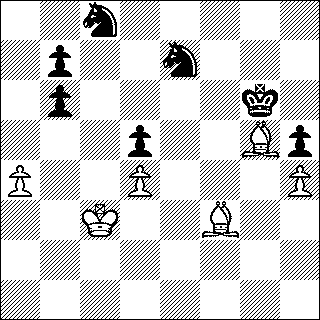
\includegraphics[width=1.5in,height=1.5in]{assets/diagrams/image96.png}

Provocando una posizione di zugzwang: comunque il Nero muova pe¢de un
pedone.

\textbf{b) Alfieri buoni e Alfieri cattivi}

Per capire se un Alfiere è buono o cattivo occorre esaminare la
disposizione dei pedoni bloccati.

Se i propri pedoni non mobili sono su casa dello stesso colore
dell'Alfiere allora l'Alfiere si dice cattivo.

\emph{diagramma 97}

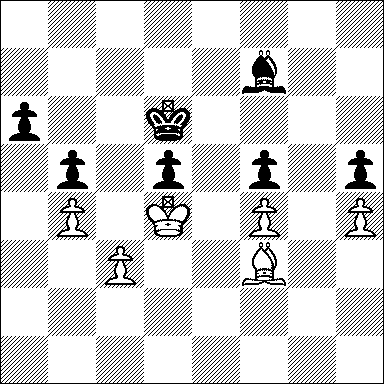
\includegraphics[width=1.40139in,height=1.40139in]{assets/diagrams/image97.png}\emph{Mossa
al Bianco}

In questa posizione, tratta da un manuale di Averbach, l'Alfiere buono
permette al Bianco di vincere nonostante il pedone in meno.

Si consideri che se la mossa fosse al Nero perderebbe subito. Una mossa
di Re permetterebbe al Bianco di penetrare (in c5 o in e5); una mossa
d'Alfiere costerebbe un pedone (il Pd5 o il Ph5). In entrambi i casi il
Nero non avrebbe più modo di difendere i rimanenti pedoni.

La mossa è però al Bianco che deve cercare di perdere un tempo,
ritornare cioè nella medesima posizione con mossa al Nero.

\textbf{1.¥e2 ¥g6} il tratto 1... ¥e8 pe¢de in modo rapido: 2.¥d3 ¥g6
(2... ¥d7 3.¥c2 ¥e6 4.¥d1 ¥f7 5.¥f3) 3.¥c2 ¥h7 4.¥b3 ¥g8 5.¥d1 ¥f7 6.¥f3
riproducendo la posizione del diagramma ma con tratto al Nero.

\textbf{2.¥d3 ¥h7} analizzando la posizione risulta chiaro che quando
l'Alfiere bianco è collocato su certe case del proprio schieramento, per
tenere la posizione il Nero deve collocare il proprio Alfiere in case
ben precise (dette case si chiamo \emph{corrispondenti}). Per esempio,
quando l'Alfiere bianco occupa la casa d3 l'Alfiere nero deve occupare
la casa f7 e, nello stesso senso, la casa d1 \emph{corrisponde} alla
casa e8.

Si osservi che nella posizione data, nella diagonale b1-h7 il Bianco
dispone di tre case mentre il Nero solo di due. Ecco allora come si può
vince la partita:

\textbf{3.¥c2 ¥g6 4.¥b1! ¥h7 5.¥d3 ¥g6 6.¥c2 ¥h7 7.¥b3} forza il Nero a
giocare l'Alfiere in una casa non corrispondente. A b3 corrisponde,
infatti, f7.

\textbf{7... ¥g8 8.¥d1 ¥f7 9.¥f3!} e si ritorna alla posizione del
diagramma con tratto al Nero. Il lettore studi bene questo istruttivo
finale.

Per far capire a un amico scacchista come gli Alfieri buoni o cattivi
possono condizionare l'intera partita un giorno, in occasione di alcune
partite lampo, gli giocai più volte questa apertura:

\textbf{1.e4 d6 2.d4 e5?!} inutile cercare questa mossa nei libri di
teoria, non c'è. Ma io inseguivo una certa idea~\ldots{}

\textbf{3.£xe5 £xe5 4.£xd8+ ¢xd8 5.¤f3 f6 6.¥e3 ¥e6 7.¤c3 c6 8.0-0-0+
¢c7} poi giocavo ¥b4-a5-b6 e cambiavo gli Alfieri su casa nera. Infine,
cambiate le Torri entravo ineluttabilmente in un finale superiore.
Insomma, nonostante l'apertura debole e lo svantaggio di tempi finivo
sempre per avere l'iniziativa.

Il trucco stava tutto in quel cambio di Alfiere. Dopo le prime mosse
sulla scacchiera si producono due pedoni bloccati: il Pe4 e il Pe5,
dunque l'Alfiere delle case nere è buono per il Bianco e cattivo per il
Nero. L'Alfiere che il Bianco deve cambiare è piuttosto quello delle
case bianche; ma il mio amico, più attento al materiale che
all'applicazione di principi di strategia, considerava quel cambio come
neutro anziché come il motivo dominante dell'intera partita.

\textbf{c) Alfieri di colore contrario}

Occorre valutare sempre con la massima attenzione un cambio che conduca
a possedere un Alfiere per parte posti su casa di colore diverso. In
tali casi le probabilità di patta aumentano e svantaggi di materiale,
anche consistenti, possono non essere decisivi.

Di norma chi è in svantaggio di materiale deve evitare di cambiare i
pezzi perché a mano a mano che ci si avvicina al finale il suo
svantaggio cresce. Quello degli Alfieri di colore contrario, è un caso
atipico: chi è in svantaggio ha convenienza ad entrare in finale, in
genere patto perché la parte più debole può bloccare il pedone su case
di colore del proprio Alfiere. L'Alfiere avversario non è infatti in
grado di sostenerne l'avanzata né di scacciare l'eventuale Re
bloccatore.

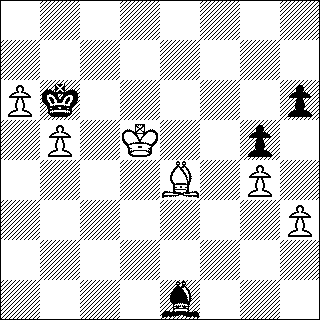
\includegraphics[width=1.5in,height=1.5in]{assets/diagrams/image98.png}

\emph{diagramma 98}

In questa posizione (di Pachman) i tre pedoni in più del Bianco non sono
sufficienti a vincere! Vediamo:

\textbf{1.¢e6 ¥g3 2.¢f6 ¥h4!} 2... ¥f4?? 3.h4! e vince.

\textbf{3.¥f3 ¢a7 4.¢e6 ¢b6 5.¢d7 ¥g3 6.¢c8 ¥f2} 6... ¥f4?? 7.h4

\textbf{7.¥c6 ¥g3 8.¥d7 ¥f2 9.¢b8 ¥g3+ 10.¢a8 ¥f2 11.a7 ¥g3 12.¥c6 ¥f2}
il nero deve sorvegliare la casa h4.

\textbf{13.¢b8 ¥g3+} patta.

Rifugiarsi negli Alfieri di colore contrario è, dunque, l'ultima
possibilità per salvare una posizione altrimenti persa. È quel che
riuscii a fare contro il Maestro Fide Mario Cocozza di Napoli, nel
torneo di Alba Adriatica del giugno 1992.

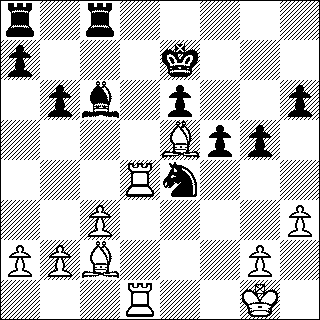
\includegraphics[width=1.5in,height=1.5in]{assets/diagrams/image99.png}In
questa partita, che illustra molto bene il comportamento da tenere in
caso di Alfieri di colore contrario, avevo perso un pedone in apertura
ma il Nero aveva dovuto rinunciare al suo Alfiere migliore e aveva
qualche difficoltà a completare lo sviluppo. Per quanto cercassi di
incrementare l'iniziativa mi rendevo ben conto che se non avessi
ottenuto un qualche compenso prima che Cocozza si fosse liberato dalla
stretta avrei perso la partita.

\emph{diagramma 99}

Alla 32\textsuperscript{a} mossa, proprio quando il Nero era ormai
prossimo a liberarsi dalla stretta, colsi al volo l'occasione di entrare
in una partita con gli Alfieri di colore contrario.

\textbf{32.¥xe4 fxe4} decisione dettata dal desiderio di crearsi un
pedone libero avanzato.

\textbf{33.¦f1} prima di procedere occorre formulare un piano. I pedoni
vanno messi su case di colore diverso dall'Alfiere avversario così che
non possano subire attacchi e per pattare occorre cambiare le Torri.
Mettere le Torri su le colonne aperte è il miglior modo per cambiarle.
In realtà ogni cambio favorisce la difesa.

\textbf{33... ¥d5 34.¦e1 b5} viene da sé che il Nero non si è creato un
pedone libero per cambiarlo col Pa2.

\textbf{35.a3 ¦f8 36.¦d2} cambiare i pezzi sì, ma non al costo della
colonna. Dopo questa mossa il Bianco minaccia il cambio perché è pronto
a contrastare la colonna con ¦f2.

\textbf{36... ¦f5 37.¥d4} il cambio è ancora sconsigliato. Il Nero,
infatti, si sdoppierebbe i pedoni e il Pe6 andrebbe a fare massa con gli
altri sul lato di Re.

\textbf{37... a6 38.¦f2 ¦g8 39.¦ef1 ¦xf2 40.¦xf2} e una!

\textbf{40... h5} minacciando la noiosa spinta in g4.

\textbf{41.¥c5+} per guadagnare un po' di tempo sull'orologio.

\textbf{41... ¢d7 42.g3!} per chiudere la porta in caso di 42... g4 con
43.h4; e tutti i pedoni bianchi finiscono su casa di colore diverso da
quella dell'Alfiere nero. Inoltre anche la spinta in h4 non è buona per
il Nero. Dopo 42... h4 43.g4 la debolezza del Pg5 gli paralizzerebbe la
Torre.

\textbf{42... ¢c6 43.¥d4 ¥c4 44.¥e3 a5 45.g4} la spinta in b5-b4
richiede la mobilitazione di tutte le forze nere ma la debolezza del Pg5
non permette alla Torre di entrare in gioco ma il Nero ha anche un altro
piano di gioco.

\textbf{45... hxg4 46.hxg4 a4} questa mossa rivela il piano del Nero:
entrare con il Re nello schieramento bianco ad ovest tramite le case
bianche (d5-c4-b3).

\textbf{47.¦h2} il Bianco si appresta ad attaccare il Pg5 con la Torre,
variante che forzerà il cambio delle Torri. Si rifletta su come ogni
mossa sia coerente col piano formulato all'inizio del finale. Avendo a
mente gli obiettivi strategici da conseguire ogni mossa appare naturale
e conseguente.

\textbf{47... ¥d3 48.¢g2 ¢d5 49.¦h5 ¥e2 50.¦xg5+ ¦xg5 51.¥xg5} e due!
Gli obiettivi strategici proposti sono stati infine conseguiti. Per
questa ragione, dopo quasi sei ore di gioco ininterrotto, commisi
l'errore di rilassarmi, considerando la partita ormai patta e finii
sull'orlo del precipizio.

\textbf{51... ¢c4 52.¥e3 ¥xg4 53.¢f2 e5 54.¥a7} felice di aver raggiunto
gli obiettivi proposti mi dimenticai dell'adagio che una patta non è
tale finché la partita non è terminata. Qui occorreva chiedersi quale
disposizione dei pezzi garantiva la patta. Non sarebbe stato difficile
scoprire che con mettendo il Re in e1 (o e3) e facendo oscillare
l'Alfiere tra b4 e f8, anche non curandosi dei pedoni b2 e c3, il Nero
non sarebbe passato.

54... ¢d3 55.¥c5 ¢d2 56.¥b6 ¥e6 57.¥c5 ¥c4 58.¥e3+ ¢c2 59.¥c5 ¢d3 60.¥b6
¢d2 61.¥a7 b4

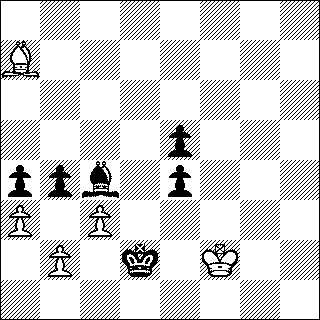
\includegraphics[width=1.33472in,height=1.33472in]{assets/diagrams/image100.png}\emph{diagramma
100}

Solo ora mi resi conto di che cosa stava tramando il Nero! Questa mossa
mira a interferire l'azione dell'Alfiere sulle diagonali a3-f8 e a1-h8.
Il Nero intende farsi scudo dei pedoni bianchi c3 e b4!

\textbf{62.¤xb4} in caso di 62.axb4? il Nero vince davvero: 62... ¢c2
63.b5 ¢xb2 64.b6 ¥d5 65.c4 ¥b7 66.¥b8 a3 67.¥xc5+ ¢b1 68.¢e3 a2 69.c5
a1=\textbf{£} 70.¥xa1 ¢xa1 71.¢d4 ¢b2 72.¢e5 d3 73.¢d6 d2 74.c6 ¥xc6
75.¢xc6 d1=\textbf{£} e vince.

\textbf{62... ¥b5} evita 63.b5.

\textbf{63.¥b6 ¢c2 64.¢e3 patta.} Infatti a 64... ¥c6 segue 65.b5 e
66.¥c5 mentre a 64... ¢xb2 65.¢xe4 ¢xa3 66.¥c7, seguita da ¥xe5 e dal
sacrificio dell'Alfiere sull'ultimo pedone nero in a1.

Invece, finché si rimane nel centro partita, specie in caso di attacchi
diretti sul Re, un Alfiere di colore contrario rafforza in modo
considerevole l'attacco perché la sua azione non può essere contrastata
dall'Alfiere avversario che opera sull'altra metà della scacchiera.

Vediamo come esempio questa partita:

Botvinnik--Pomar, Amsterdam 1966 \textbf{(Difesa Slava)}

\textbf{1. c4 c6} poiché Botvinnik è un grande esperto della partita
Inglese con questa spinta e la successiva Pomar pone le basi per un
rientro nella partita di Donna. È ovvio che il Nero deve essere pronto a
giocare una Caro Kann. Spesso in apertura si svolge una lotta so¢da per
cercare di indirizzare la partita sui binari più graditi.

\textbf{2.¤c3 d5 3.¤xd5 ¤xd5 4.d4} rompe gli indugi e rientra nella
partita di Donna.

\textbf{4... ¤f6 5.¤f3 ¤c6 6.¥f4 ¥f5 7.e3 e6 8.¥b5 ¥b4} la scelta di
mantenere a lungo la simmetria non è mai favorevole al Nero; il Bianco
trascina il tempo di vantaggio e può rompere la simmetria a piacimento.
In questi schemi le possibilità di controgioco del Nero sono minori che
in altre varianti.

\textbf{9.¤e5 £a5 10.¥xc6+ bxc6 11.0-0 ¥xc3} con questa mossa si vengono
ad avere gli Alfieri di colore contrario. Un eventuale finale di soli
Alfieri e pedoni sarebbe patto ma il Nero deve riuscire ad arrivare al
finale.

\textbf{12.bxc3} Botvinnik aveva già giocato questa variante contro Tal,
nella finale di campionato del mondo del 1961. Tal aveva continuato con
12... £xc3 13.£c1 £xc1 14.¦fxc1 con posizione favorevole al Bianco.
Pomar tenta un miglioramento.

\textbf{12... ¦c8 13.c4 0-0 14.g4} Botvinnik: \emph{``Il piano è
semplice: si spinge in c5, poi in f3, si cambia eventualmente il proprio
¤e5 con l'Alfiere nemico portandosi in g6, e si ottiene il controllo
della colonna b. Può il Nero impedire tutto ciò?''}

\textbf{14... ¥g6 15.c5 ¤e4 16.f3 ¤d2 17.¦f2 ¤c4 18.¤xc4 £xc4 19.¥d6}
l'attività dei pezzi bianchi è maggiore ma soprattutto il Bianco può
sfruttare la massa dei pedoni per guadagnare spazio sulla scacchiera. La
debolezza del \textbf{§}c4, dati gli Alfieri di colore contrario, non
sarebbe grave di per sé, se disgiunta dagli altri fattori posizionali.

\textbf{19... ¦fe8 20.e4 f5 21.£c2 fxe4 22.fxe4 £a3 23.¦e1} il vantaggio
del Bianco è netto.

\textbf{23... £h3 24.¦g2 T¤d8 25.¦g3 £h6 26.£xc4 £d2 27.£c3!}
restituisce il materiale ma ottiene un forte attacco.

\textbf{27... £xa2} l'entrata in finale con 27... £xc3 28.¦xc3 ¦d7
29.¦b3 avrebbe permesso al Bianco di vincere senza difficoltà.

\textbf{28.¦g2 £a6 29.h4 ¦d7 30.h5 ¥f7 31.¦a1 £c8 32.£f3 £d8 33.g5 g6}

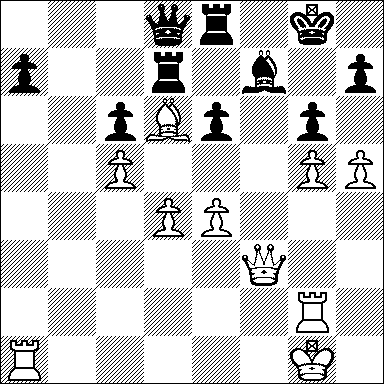
\includegraphics[width=1.40139in,height=1.40139in]{assets/diagrams/image101.png}\emph{diagramma
101}

Si noti la diversa attività dei due Alfieri. Quello bianco ha l'assoluto
dominio delle case nere, particolarmente delicate quelle intorno al Re
(f8-g7-h8) mentre quello nero è accecato. Per da¢gli un po' di luce il
Nero non esita a sacrificare un pedone.

\textbf{34.h6 e5 35.¥xe5 ¦b7 36.£f4 a5 37.¦f3 ¥b3 38.d5 ¤xd5 39.c6 ¦a7
40.c7 £e7 41.¥d6 il Nero abbandona} la minaccia di matto in f8 (una casa
nera!) costringe il Nero alla resa.
